\chapter{Bluetooth-Controlled Car}

RC (radio-controlled) cars have been a favorite toy of children. This project aims to build a car that can be controlled by a cellphone by means of Bluetooth connectivity. It is not only easy to make but fun to play with as well.

%Remote control cars have always been a source of joy for all of us since our childhood. In this demonstration we are going to make a Bluetooth-Controlled Car from scratch. The car will be connected to your mobile phone using Bluetooth. After installing a particular application in your mobile phone, you will be able to control the car through your mobile phone. 

\subsection*{Components}
\begin{table}[H]
    \centering
    \begin{tabular}{|c|l|c|}\hline
     \textbf{\#} & \textbf{Components} &  \textbf{Amount}\\\hline
     1 & L298N: Motor driver       & 1\\\hline
     2 & HC-05: Bluetooth module    & 1 \\\hline
     3 & Push buttons               & 2 \\\hline
     4 & 9V battery                 & 1 \\\hline
     5 & 12V rechargeable battery   & 1 \\\hline
     6 & Car chassis                & 1 \\\hline
     7 & Arduino UNO                & 1 \\\hline
     8 & Connecting wires           & - \\\hline
    \end{tabular}
\end{table}

\subsection*{Connections}
The circuit will need to be patched on the car. For this purpose, assemble the car chassis and connect the components as instructed below while fixing the components on the car at suitable positions on the chassis.

\begin{enumerate}[leftmargin=*]
    \item Connect Vcc and GND pin of the Bluetooth module with 5V and GND pins of Arduino respectively. 
    \item Connect Tx and Rx pins of the Bluetooth module with Rx and Tx pin of Arduino respectively. 
    \item Connect the 12 V power supply to the motor driver via a button. Also connect GND of Arduino with GND of the motor driver.
    \item Connect the 9V battery to Vin and GND pins of Arduino via a button. 
    \item Connect the control pins of the motor driver (IN1, IN2, IN3, IN4) to pins 6, 7, 8 and 9 of Arduino.
    \item Connect the output pins of the motor driver (OUT1, OUT2, OUT3, OUT4) with DC motors (fig. \ref{fig:bt-car}).
\end{enumerate}

	\begin{figure}[H]
	\centering 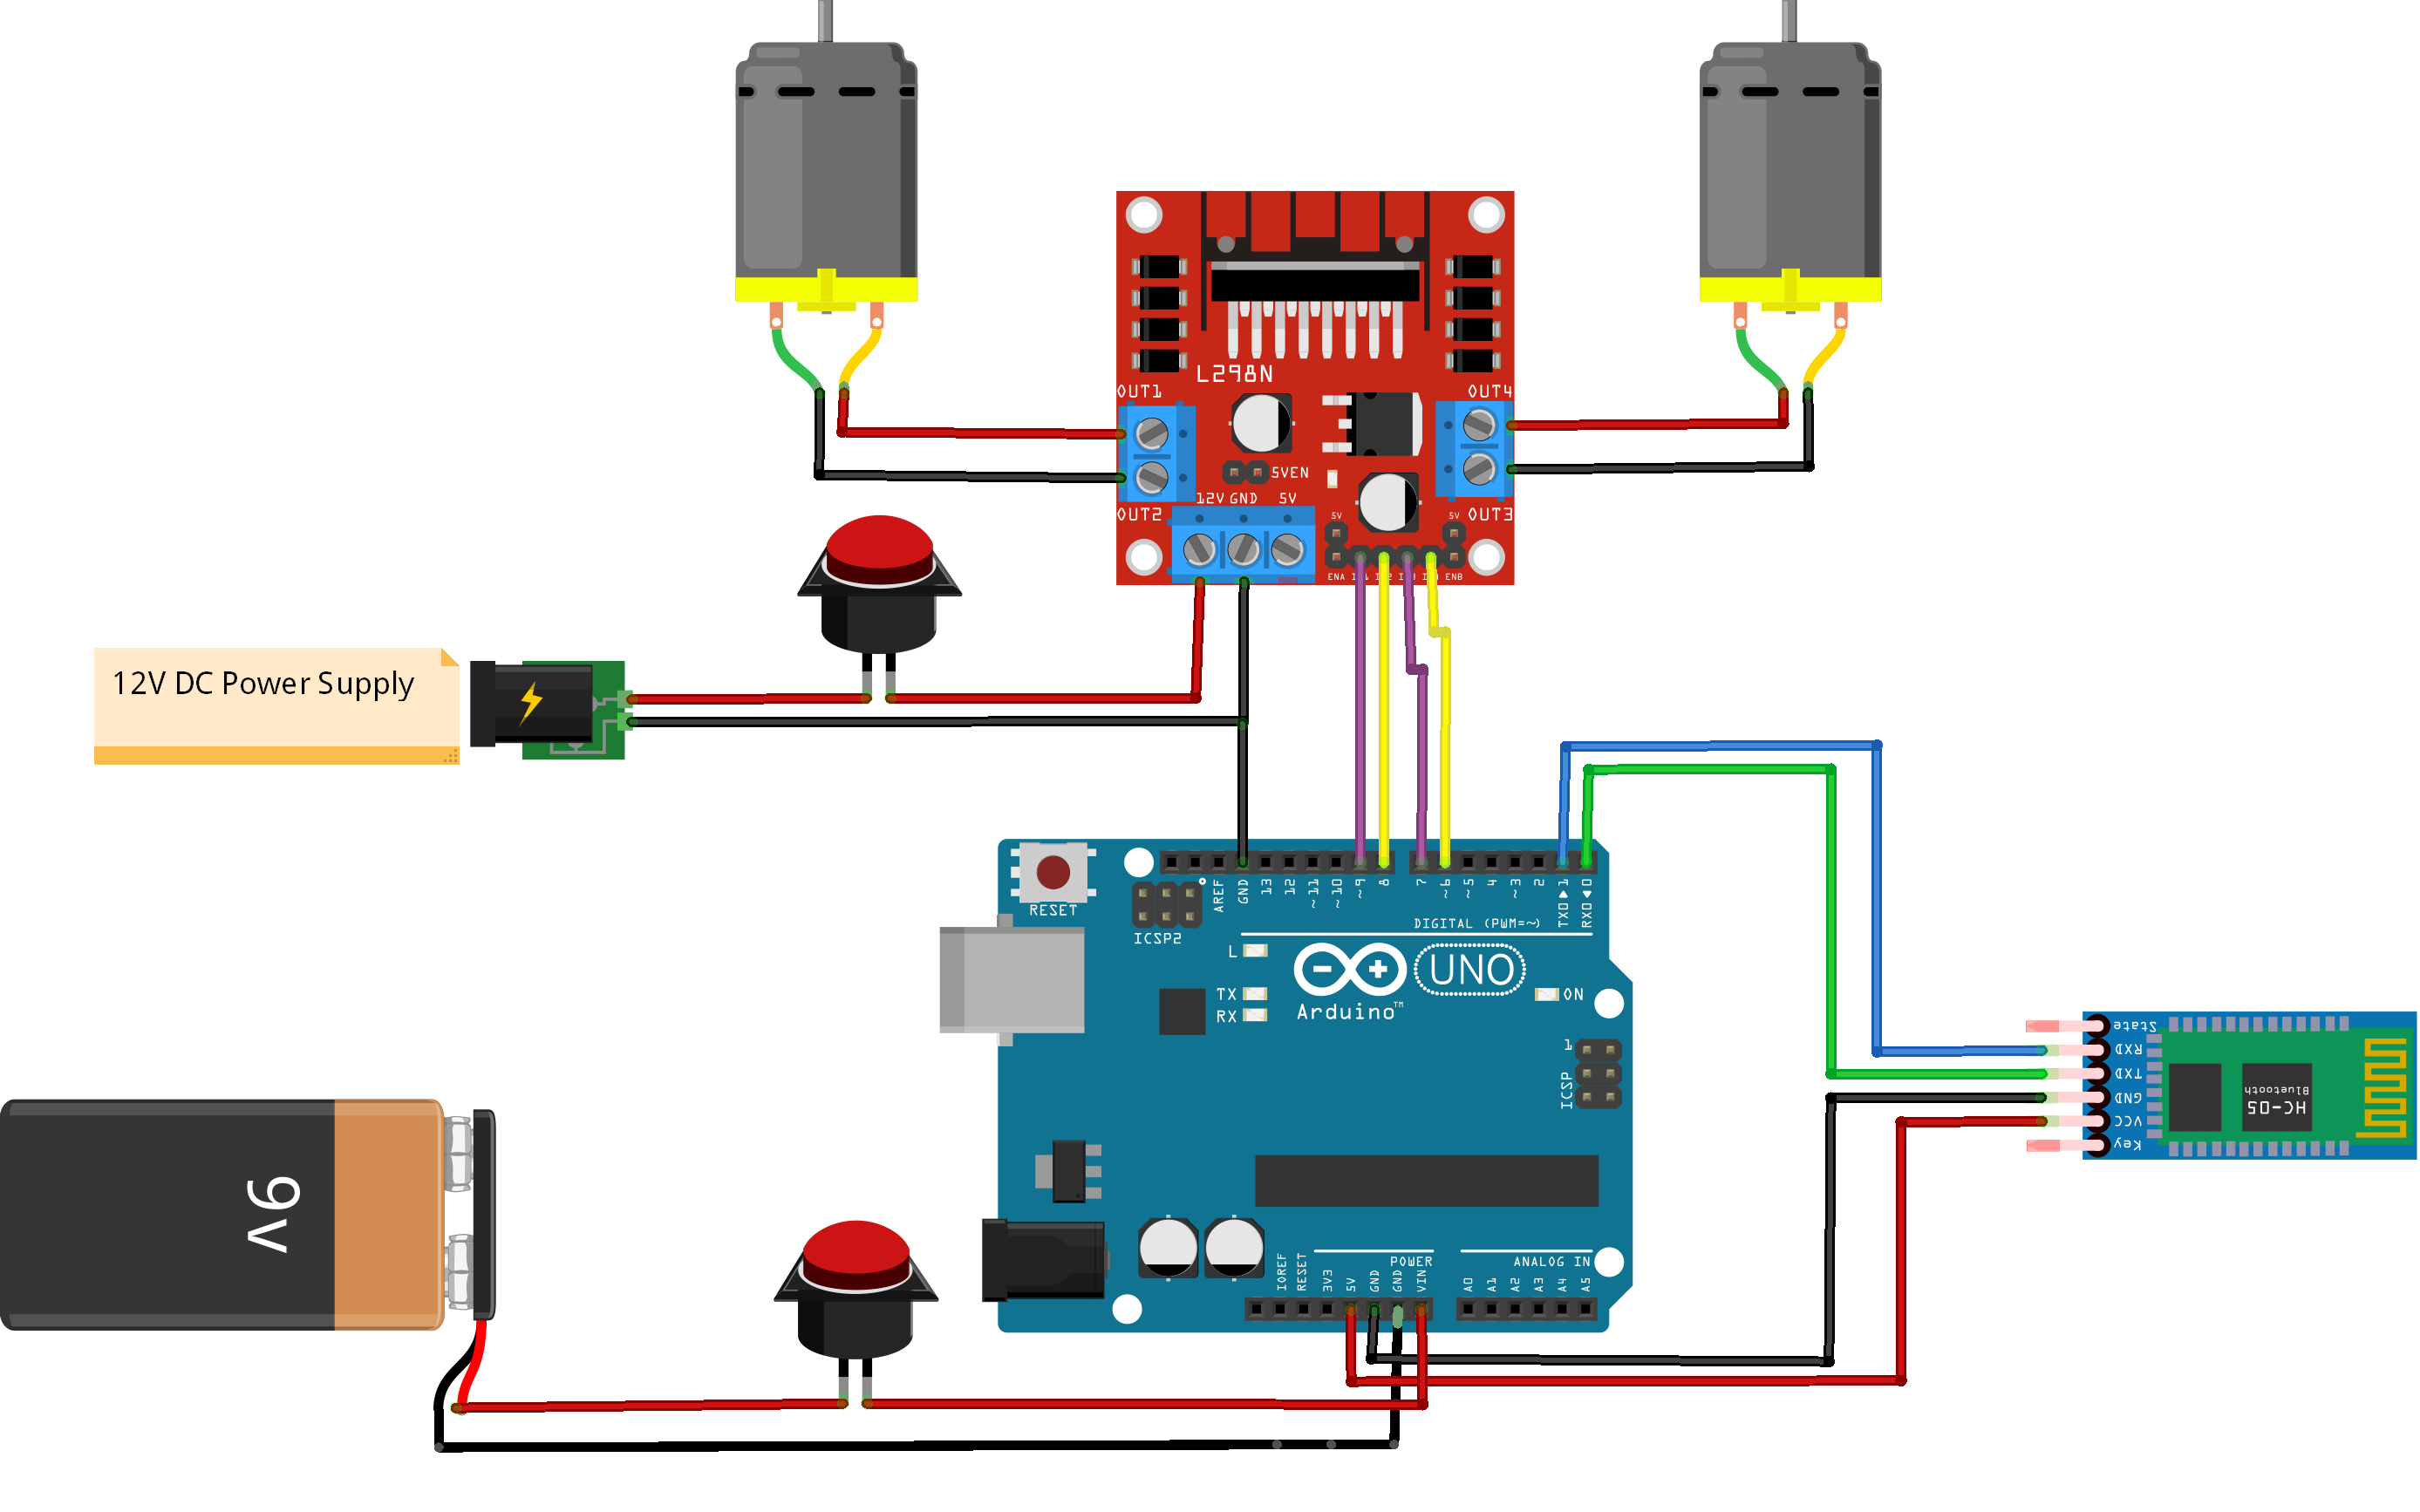
\includegraphics[width=0.7\linewidth]{recreational_exp/bluetooth car_bb.png}
	\caption{Circuit diagram of Bluetooth Car}
	\label{fig:bt-car}
	\end{figure}
	
\subsection*{Procedure}
\begin{enumerate}[leftmargin=*] 
    \item Copy lst.\ref{list:bluetooth-car} to a new Arduino sketchbook. Upload the code to your Arduino board. Remove Tx and Rx pins of the Bluetooth module while uploading the code.
    \item Turn the switch ON to supply the power to the motor.
    \item Download the app `Arduino Bluetooth RC Car' in your cellphone. 
    \item Turn on Bluetooth of your mobile. Pair with the Bluetooth module by using the default password `1234'. Now open the downloaded app and connect it with the Bluetooth module. 
    \item Control the car by using the navigation buttons on the app.  
\end{enumerate}

	
\begin{lstlisting}[language=Arduino, numbers=none, caption={Code for bluetooth-controlled car}, captionpos=b, label={list:bluetooth-car}]
// motor 1 pins 
int m11=8;
int m12=9;

// motor 2 pins
int m21=6;
int m22=7;

// variable to read data from bluetooth 
char input; // controling chracter
int spd;  // speed of the motors

// Defining functions
void forward(int dum){
  analogWrite(m11, dum);
  analogWrite(m12, LOW);
  analogWrite(m21, dum);
  analogWrite(m22, LOW);
}
void backward(int dum){
  analogWrite(m11, LOW);
  analogWrite(m12, dum);
  analogWrite(m21, LOW);
  analogWrite(m22, dum);
}
void right(int dum){
  analogWrite(m11, dum);
  analogWrite(m12, LOW);
  analogWrite(m21, LOW);
  analogWrite(m22, dum);
}
void left(int dum){
  analogWrite(m11, LOW);
  analogWrite(m12, dum);
  analogWrite(m21, dum);
  analogWrite(m22, LOW);
}
void stay (void){
  analogWrite(m11, LOW);
  analogWrite(m12, LOW);
  analogWrite(m21, LOW);
  analogWrite(m22, LOW);
}
void Fleft(int dum){
  analogWrite(m11, dum/2);
  analogWrite(m12, LOW);
  analogWrite(m21, dum);
  analogWrite(m22, LOW);
}
void Fright(int dum){
  analogWrite(m11, dum);
  analogWrite(m12, LOW);
  analogWrite(m21, dum/2);
  analogWrite(m22, LOW);
}
void Bright(int dum){
  analogWrite(m11, LOW);
  analogWrite(m12, dum);
  analogWrite(m21, LOW);
  analogWrite(m22, dum/2);
}
void Bleft(int dum){
  analogWrite(m11, LOW);
  analogWrite(m12, dum/2);
  analogWrite(m21, LOW);
  analogWrite(m22, dum);
}


void setup() {
  // put your setup code here, to run once:
Serial.begin(9600);
pinMode(m11, OUTPUT);
pinMode(m12, OUTPUT);
pinMode(m21, OUTPUT);
pinMode(m22, OUTPUT);
}

void loop() {
  if(Serial.available()>0){
    input= Serial.read();
    Serial.println(input);

    if (input>='0' && input<='9')
       {
        spd=55+(input-47)*20;
       }
    else if(input == 'F'){
      forward(spd);
    }
    else if(input == 'B'){
      backward(spd);
    }
    else if(input == 'L'){
      left(spd);
    }
    else if(input == 'R'){
      right(spd);
    }
    else if(input == 'G'){
      Fleft(spd);
    }
    else if(input == 'I'){
      Fright(spd);
    }
    else if(input == 'H'){
      Bleft(spd);
    }
    else if(input == 'J'){
      Bright(spd);
    }
    else{
      stay();
    }
 }
}
\end{lstlisting}

\subsection*{Precautions}
\begin{itemize}[leftmargin=*] 
    \item Do not forget to remove Tx and Rx pins of the Bluetooth module from the Arduino board while uploading the code.
    \item If multiple Bluetooth modules are present at the location, it may create problem in connecting with the required Bluetooth module because all Bluetooth modules have the same password by default. To resolve this issue, AT mode of the Bluetooth module can be used.
    \item If the car is not moving according to the transmitted commands, try swapping the control pins of the motor driver.
\end{itemize}